\chapter{\textbf{RESULTADOS E DISCUSSÃO}}
Este capítulo apresenta os resultados das simulações e análises estruturadas para avaliar o impacto do Art. 36 da Portaria MTP nº 1.467/2022 sobre as PM. Inicialmente, são detalhadas as quatro massas seguradas construídas, cujas distribuições etárias distintas servem de base para testar a sensibilidade do critério normativo. Em seguida, são apresentados os resultados das PM para cada método de custeio em cada perfil etário simulado, seguidos dos fatores explicativos desses resultados.

\section{\textbf{Massas seguradas}}
Nesta seção, detalham-se as características demográficas das quatro massas populacionais simuladas para este estudo. Cada base de dados foi composta por um contingente de $100.000$ segurados, distribuídos entre homens e mulheres. Essas quatro massas populacionais simuladas são evidenciadas na Figura \ref{fig:piramides}.

\begin{figure}[H]
    \centering
    \singlespacing\caption{Comparação das Pirâmides Etárias das Populações Simuladas}
    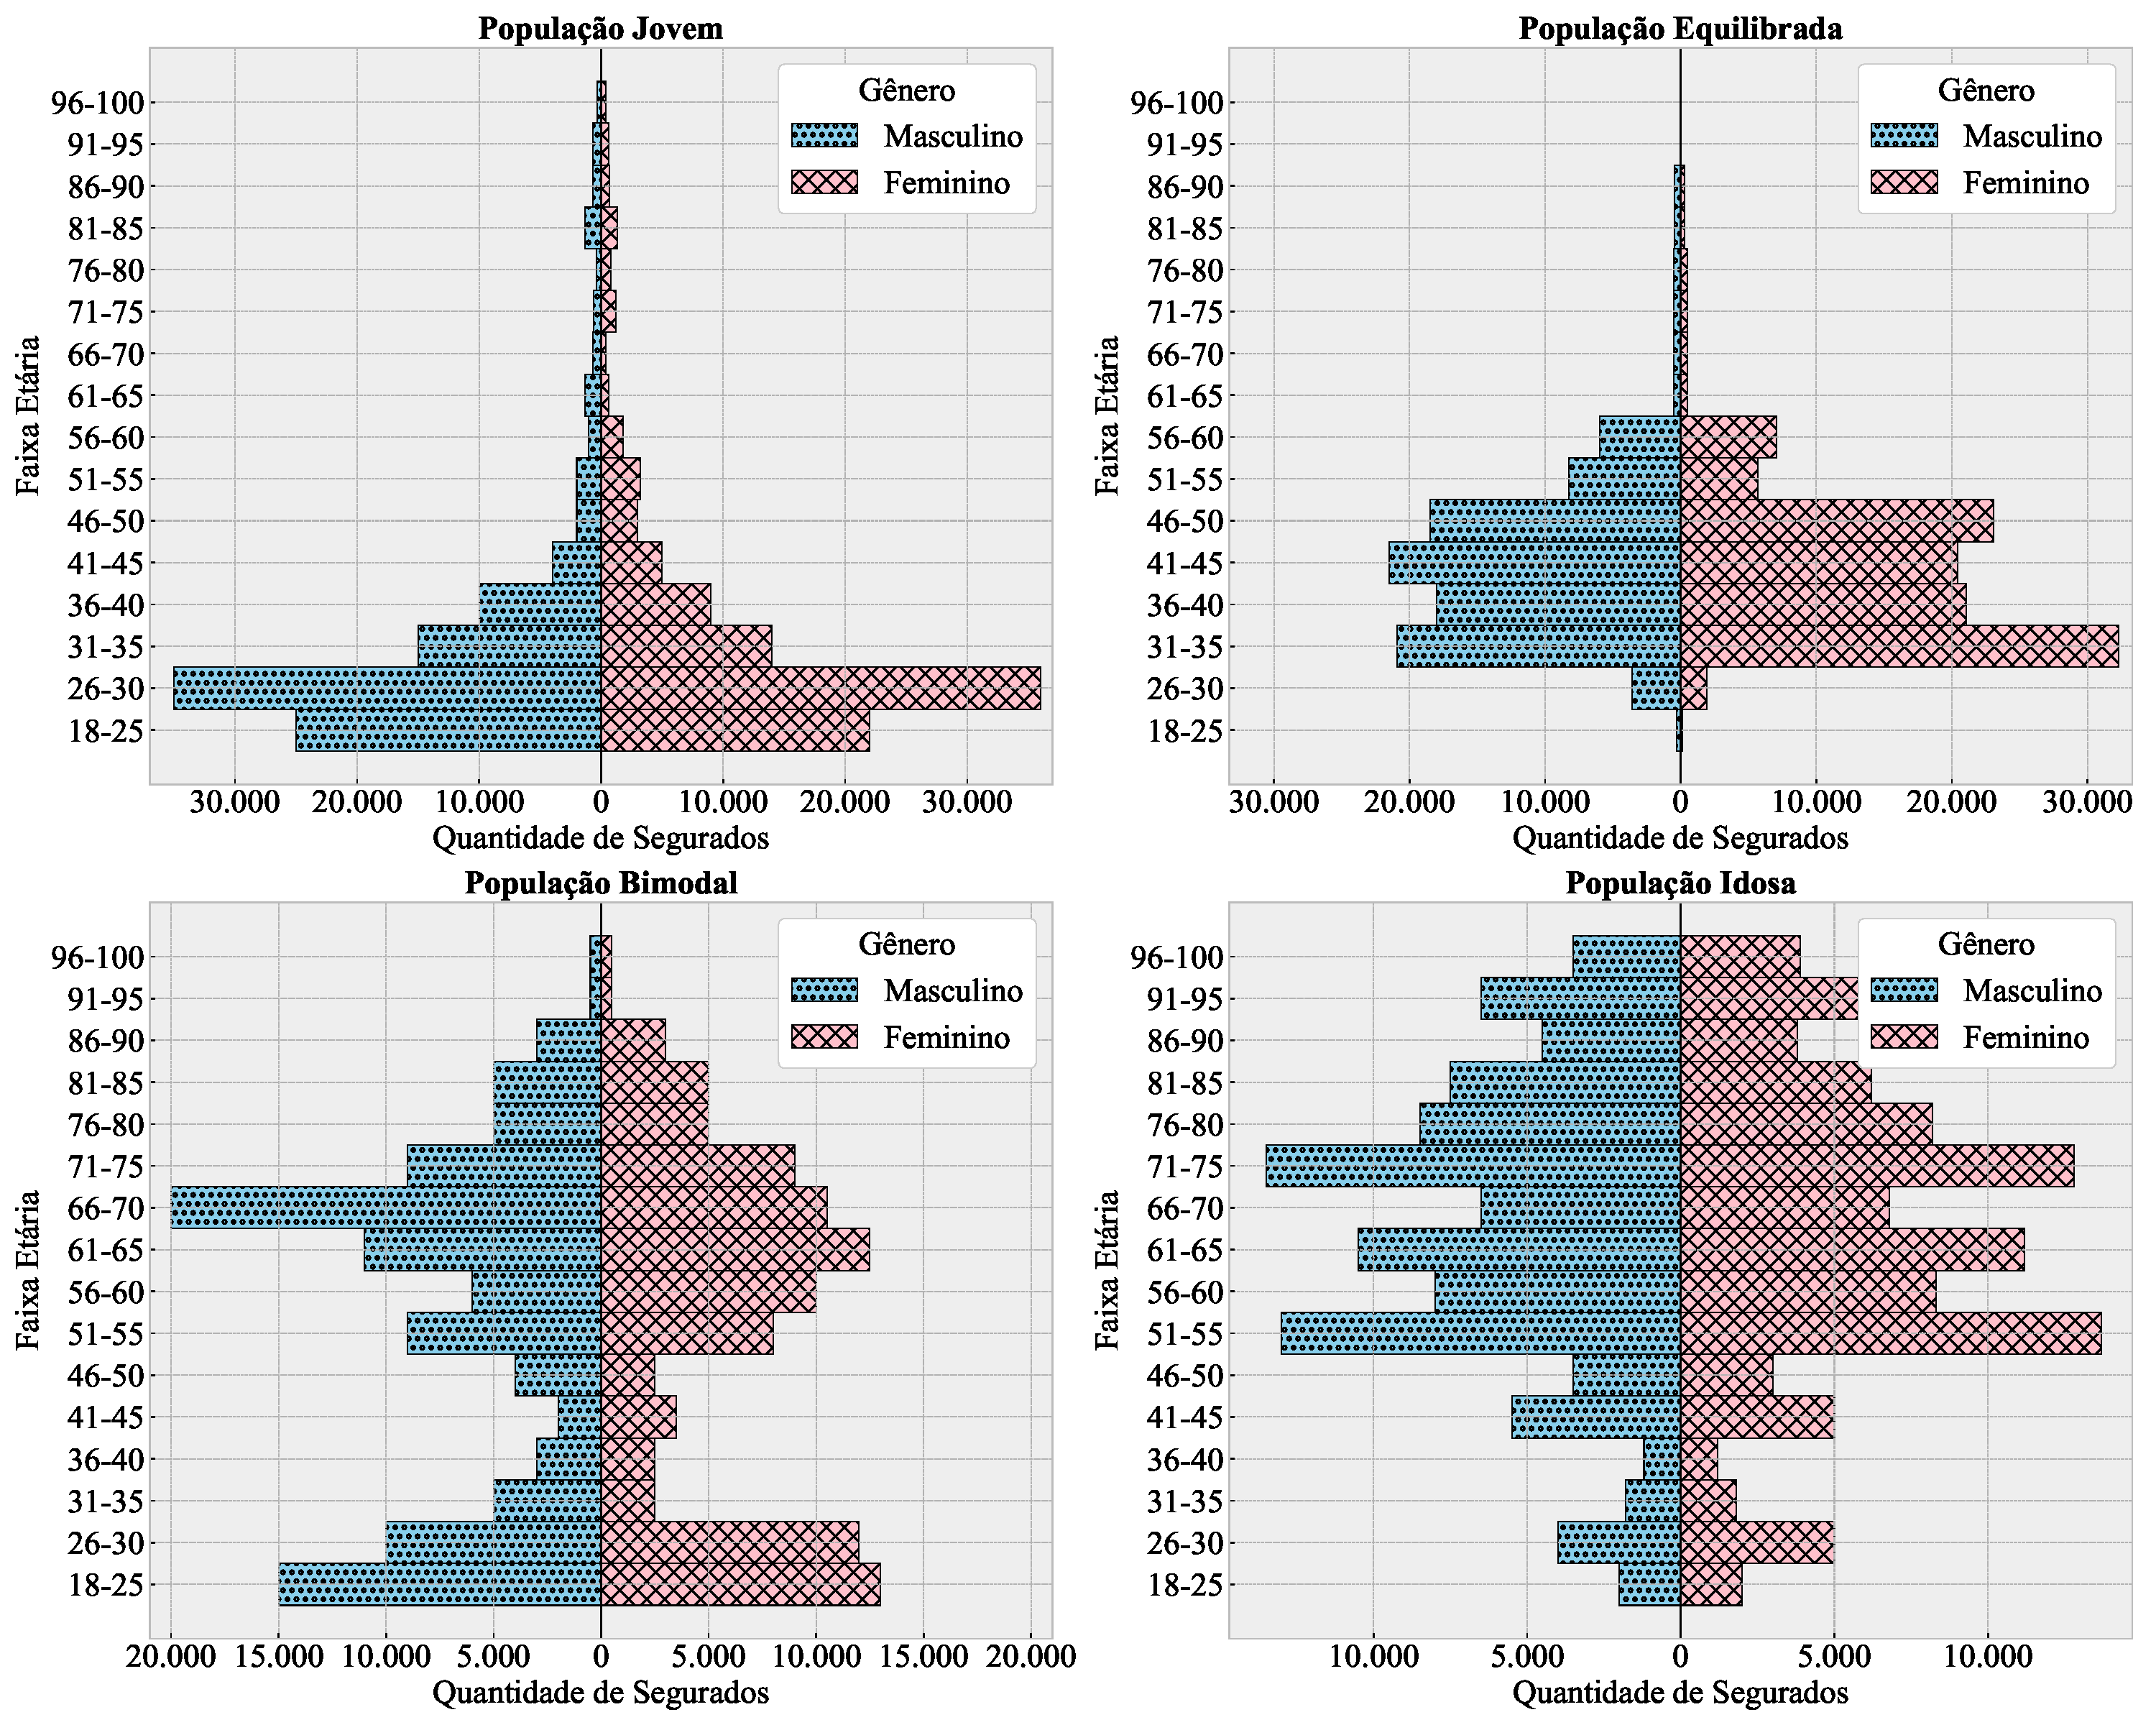
\includegraphics[width=0.97\textwidth]{piramides_etarias.pdf}
    \fonte{Elaboração própria (2026).}
    \label{fig:piramides}
\end{figure}

O perfil jovem simulado é evidênciado com a pirâmide etária superior esquerda contida na Figura \ref{fig:piramides}. A maior concentração de segurados encontra-se nas faixas de 18 a 30 anos, que representam aproximadamente $60\%$ da população masculina e $58\%$ da feminina. A massa equilibrada, representada pela pirâmide superior direito na Figura \ref{fig:piramides} possui uma distribuição mais homogênea, com concentrações relevantes nas faixas centrais (entre 31 e 50 anos). Para as mulheres, observa-se um pico significativo na faixa de 31-35 anos ($32,3\%$), enquanto os homens apresentam uma distribuição mais plana entre os 31 e 50 anos.

O perfil idoso mostrada na pirâmide inferior direita da Figura \ref{fig:piramides} representa um regime com ausência prolongada de novos concursos, esta massa concentra a maioria de seus segurados acima dos 51 anos. Notavelmente, as faixas de 71-75 anos e de 91-95 anos apresentam pesos significativos. A massa bimodal, evidenciada pela pirâmide inferior esquerda da Figura \ref{fig:piramides}, representa o cenário de um RPPS que passou por um longo período de interrupção de contratações, seguido por um certame recente de grande porte.

A Tabela \ref{tab:estatisticas_descritivas} apresenta as principais estatísticas  descritivas das quatro massas seguradas simuladas. O indicador de maturidade da  massa, definido como a razão entre o número de segurados em fase contributiva  (homens com idade inferior a 65 anos e mulheres com idade inferior a 62 anos) e  o número de segurados em fase de percepção de benefícios, sintetiza o grau de  equilíbrio demográfico de cada base.

\vspace{0.25cm}
\begin{table}[htbp]
    \centering
    \caption{Estatísticas Descritivas das Massas Seguradas Simuladas}
    \renewcommand{\arraystretch}{1.2}
    \begin{tabular}{lrrrr}
    \toprule
    \multicolumn{1}{c}{\textbf{Estatística}} & \multicolumn{1}{c}{\textbf{Jovem}} & \multicolumn{1}{c}{\textbf{Equilibrada}} & \multicolumn{1}{c}{\textbf{Bimodal}} & \multicolumn{1}{c}{\textbf{Idosa}} \\
    \midrule
    Idade Média              & 33,57  & 42,54  & 54,15  & 65,13  \\
    Idade Mediana            & 29,00  & 42,00  & 59,00  & 65,00  \\
    Idade Mínima             & 19,00  & 19,00  & 19,00  & 19,00  \\
    1º Quartil               & 26,00  & 35,00  & 32,00  & 53,00  \\
    2º Quartil               & 29,00  & 42,00  & 59,00  & 65,00  \\
    3º Quartil               & 36,00  & 48,00  & 70,00  & 78,00  \\
    Idade Máxima             & 100,00 & 100,00 & 100,00 & 100,00 \\
    Maturidade da Massa      & 17,44  & 41,18  &  1,35  &  0,81  \\
    \bottomrule
    \end{tabular}
    \label{tab:estatisticas_descritivas}
    \vspace{0.25cm}
    \fonte{Elaboração própria (2026).}
\end{table}

A base jovem, com idade média de $33{,}57$ anos e mediana de $29{,}00$ anos, apresenta a maior assimetria positiva entre as duas medidas de tendência central, indicando que uma parcela de segurados em idades mais avançadas eleva a média acima da concentração efetiva da distribuição. O 1º e o 3º quartis, de $26$ e $36$ anos respectivamente, confirmam a forte concentração nas faixas etárias mais jovens. O indicador de maturidade de $17{,}44$ revela que, para cada segurado em fase de benefício, existem aproximadamente $17$ segurados em fase contributiva, configurando um cenário de expressiva folga financeira e baixa pressão imediata sobre o passivo.

A base equilibrada, ainda que apresente uma razão de maturidade superior ($41{,}18$), registra idade média de $42{,}54$ anos e a maior simetria entre média e mediana ($42{,}54$ e $42{,}00$, respectivamente), com amplitude interquartílica de $13$ anos (entre $35$ e $48$ anos). A elevada maturidade decorre da concentração etária nas faixas centrais, que ainda se situam predominantemente abaixo dos limiares de aposentadoria, resultando em reduzida massa de beneficiários em termos absolutos.

A base bimodal apresenta as características mais distintas do conjunto. A amplitude interquartílica de $38$ anos --- do 1º quartil de $32$ anos ao 3º quartil de $70$ anos --- é a maior entre as quatro massas e reflete a estrutura com dois grupos populacionais bem definidos, um grupo de segurados jovens recentemente ingressos e um grupo idoso em iminente ou já concedida aposentadoria. A diferença entre mediana ($59{,}00$) e média ($54{,}15$) indica que o grupo jovem, embora numericamente relevante, não é suficiente para deslocar a mediana para abaixo dos $50$ anos. O indicador de maturidade de $1{,}35$ sinaliza que a base já se encontra próxima ao equilíbrio entre ativos e inativos, com ligeira predominância contributiva.

Por fim, a base idosa apresenta a maior idade média ($65{,}13$ anos) e a maior coincidência entre média e mediana, indicando uma distribuição etária praticamente simétrica em torno de uma faixa de alta senioridade. Com 1º quartil de $53$ anos e 3º quartil de $78$ anos, a massa apresenta baixíssima presença de segurados jovens. O indicador de maturidade de $0{,}81$ é o único inferior à unidade, confirmando que a base idosa é a única em que os beneficiários já superam numericamente os contribuintes, caracterizando o cenário de maior pressão sobre o passivo atuarial e de maior sensibilidade às premissas de mortalidade nas idades avançadas.

\section{\textbf{Provisões matemáticas e inconsistências}}

Esta seção apresenta os resultados das provisões matemáticas calculadas de acordo com as premissas contidas no Quadro \ref{qua:hipoteses_atuariais}. Para cada base de dados simulada, foram calculadas as PM segundo os métodos de custeio INE, CUP e PNI, confrontando-se cada tábua comparativa com a tábua de referência. Uma tábua é classificada como inconsistente quando apresenta expectativa de vida na idade média superior à da tábua de referência e, concomitantemente, produz uma PM inferior à gerada pela tábua de referência.

% --------------------- Base Jovem --------------------------------------
As Tabelas \ref{tab:jovem-ine}, \ref{tab:jovem-CUP} e \ref{tab:jovem-pni} apresentam, respectivamente, os resultados para a base jovem nos métodos INE, CUP e PNI. Em todos os casos, a primeira linha de cada gênero corresponde à tábua de referência (IBGE 2024 Extrapolada), cujo valor de PM serve de parâmetro para identificar as inconsistências. As demais tábuas contidas nessas tabelas registraram uma PM inferior àquela gerada pela tábua de referência. Além disso, são apresentadas as respectivas expectativas de vida na idade média associadas a cada tábua.
\vspace{0.25cm}
\begin{table}[htbp]
    \centering
    \caption{Provisões Matemáticas - Base Jovem - Método INE}
    \begin{threeparttable}
    \renewcommand{\arraystretch}{1.0}
    \begin{tabular}{llrr}
    \toprule
    \multicolumn{1}{c}{\textbf{Gênero}} & \multicolumn{1}{c}{\textbf{Tábua}} & \multicolumn{1}{c}{\textbf{PM}} & \multicolumn{1}{c}{\textbf{$e_{33}$}} \\ \midrule
    \multirow{11}{*}{Masculino} & IBGE 2024 Extrapolada Masculina & 45.598.237,44	& 43,55 \\
                                & IBGE 2019 Extrapolada Ambos Agravada em 19\% & 45.534.229,61 & 43,60 \\
                                & AT-2000 Masculina Agravada em 33\% & 44.909.930,94 & 44,14 \\
                                & AT-55 & 43.848.527,38 & 43,60 \\
                                & AT-55 Suavizada em 5\% & 44.906.722,62 & 44,15 \\
                                & AT-83 Basic Masculina & 44.396.709,59 & 44,13 \\
                                & AT-83 Basic Masculina Suavizada em 2,5\% & 44.896.625,32 & 44,39 \\
                                & BR-EMSmt-v.2021 Masculina Agravada em 24\% & 44.994.744,87 & 44,05 \\
                                & GKM-95 & 43.927.302,57 & 43,59 \\
                                & Prudential-50 Suavizada em 16\% & 45.585.859,77 & 44,26 \\ 
                                & M-95 H Suavizada em 6\% & 44.714.222,92 & 43,95 \\ \hline
    \multirow{4}{*}{Feminino} & IBGE 2024 Extrapolada Feminina & 66.937.295,03	 & 48,70 \\
                                & BR-EMSmt-v.2021 Feminina Agravada em 21,5\% & 66.839.871,57 & 48,84 \\
                                & GAM-71 Feminina & 66.551.189,09 & 48,87 \\
                                & Petros Suavizada em 13\% & 66.228.077,79 & 48,71 \\ \bottomrule
    \end{tabular}
    \begin{tablenotes}[flushleft]
        \small
        \item Fonte: Elaboração própria (2026).
    \end{tablenotes}
    \end{threeparttable}
    \label{tab:jovem-ine}
\end{table}
\vspace{0.5cm}
\begin{table}[htbp]
    \centering
    \caption{Provisões Matemáticas - Base Jovem - Método CUP}
    \begin{threeparttable}
    \renewcommand{\arraystretch}{1.0}
    \begin{tabular}{llrr}
    \toprule
    \multicolumn{1}{c}{\textbf{Gênero}} & \multicolumn{1}{c}{\textbf{Tábua}} & \multicolumn{1}{c}{\textbf{PM}} & \multicolumn{1}{c}{\textbf{$e_{33}$}} \\ \midrule
    \multirow{9}{*}{Masculino} & IBGE 2024 Extrapolada Masculina & 33.299.758,59	& 43,55 \\
                    & AT-2000 Masculina Agravada em 33\% & 32.678.511,80 & 44,14 \\
                    & AT-55 & 32.048.662,32	& 43,60 \\
                    & AT-55 Suavizada 5\% & 32.825.920,09 & 44,15 \\
                    & AT-83 Basic Masculina & 32.327.043,98 & 44,13 \\
                    & AT-83 Basic Masculina Suavizada 2,5\% & 32.694.946,44 & 44,39 \\
                    & BR-EMSmt-v.2021 Masculina Agravada em 24\% & 32.776.498,80 & 44,05 \\
                    & GKM-95 & 32.032.418,81 & 43,59 \\
                    & M-95 H Suavizada 6\% & 32.536.096,19 & 43,95 \\ \hline
    \multirow{4}{*}{Feminino} & IBGE 2024 Extrapolada Feminina & 49.671.069,71 & 48,70 \\
                                & BR-EMSmt-v.2021 Feminina Agravada em 21,5\% & 49.654.760,02 & 48,84 \\
                                & GAM-71 Feminina & 49.246.868,07 & 48,87 \\ 
                        & Petros Suavizada 13\% & 49.121.704,09 & 48,71 \\ \bottomrule
    \end{tabular}
    \begin{tablenotes}[flushleft]
        \small
        \item Fonte: Elaboração própria (2026).
    \end{tablenotes}
    \end{threeparttable}
    \label{tab:jovem-CUP}
\end{table}

\begin{table}[htbp]
    \centering
    \caption{Provisões Matemáticas - Base Jovem - Método PNI}
    \begin{threeparttable}
    \renewcommand{\arraystretch}{1.0}
    \begin{tabular}{llrr}
    \toprule
    \multicolumn{1}{c}{\textbf{Gênero}} & \multicolumn{1}{c}{\textbf{Tábua}} & \multicolumn{1}{c}{\textbf{PM}} & \multicolumn{1}{c}{\textbf{$e_{33}$}} \\ \midrule
    \multirow{13}{*}{Masculino}
    & IBGE 2024 Extrapolada Masculina                  & 30.208.928,00 & 43,55 \\
    & IBGE 2019 Extrapolada Ambos Agravada em 19\%      & 29.866.462,94 & 43,60 \\
    & IBGE 2019 Extrapolada Ambos Agravada em 18,3\%    & 29.976.475,14 & 43,70 \\
    & AT-2000 Masculina Agravada em 33\%               & 28.611.697,60 & 44,14 \\
    & AT-55                               & 27.915.473,47 & 43,60 \\
    & AT-55 Suavizada em 5\%                     & 28.575.622,26 & 44,15 \\
    & AT-83 Basic Masculina                       & 27.976.902,86 & 44,13 \\
    & AT-83 Basic Masculina Suavizada em 2,5\%           & 28.290.738,39 & 44,39 \\
    & BR-EMSmt-v.2021 Masculina Agravada em 24\%        & 28.974.636,30 & 44,05 \\
    & GKM-95                              & 28.451.524,37 & 43,59 \\
    & Prudential-50 Suavizada em 16\%            & 29.189.236,82 & 44,26 \\
    & TR 2025                             & 29.985.619,04 & 43,84 \\
    & M-95 H Suavizada em 6\%                    & 28.925.074,93 & 43,95 \\ \hline
    \multirow{5}{*}{Feminino}
    & IBGE 2024 Extrapolada Feminina                  & 40.739.430,62 & 48,70 \\
    & BR-EMSmt-v.2021 Feminina Agravada em 21,5\%     & 40.676.942,28 & 48,84 \\
    & GAM-71 Feminina                            & 39.948.430,84 & 48,87 \\
    & GAM-71 Feminina Suavizada em 5\%                   & 40.556.722,03 & 49,36 \\
    & Petros Suavizada em 13\%               & 39.854.702,97 & 48,71 \\ \bottomrule
    \end{tabular}
    \begin{tablenotes}[flushleft]
        \small
        \item Fonte: Elaboração própria (2026).
    \end{tablenotes}
    \end{threeparttable}
    \label{tab:jovem-pni}
\end{table}
\FloatBarrier
A base jovem é a mais suscetível à ocorrência de inconsistências dentre as quatro bases analisadas. Nos métodos INE e CUP, verificam-se 10 e 8 tábuas inconsistentes para o sexo masculino, respectivamente, e 3 tábuas para o sexo feminino em ambos os métodos. Os métodos INE e CUP compartilham as mesmas tábuas inconsistentes para o sexo feminino, diferindo apenas na composição masculina e, naturalmente, nos valores absolutos das provisões.

A análise dos valores absolutos revela que os desvios em relação à tábua de referência podem apresentar níveis mais elevados no gênero masculino. No método INE, a tábua AT-55 masculina produz uma PM de R\$43.848.527,38, o que representa uma redução de aproximadamente 3,8\% em relação à referência. A tábua GKM-95 apresenta uma magnitude similar, enquanto as tábuas AT-83 Basic masculina e AT-2000 masculina agravada em 33\% ficam cerca de 2,6\% abaixo da referência. Para o sexo feminino, as reduções são relativamente menores em termos percentuais, com a tábua Petros suavizada 13\% registrando um desvio de aproximadamente 1,1\% abaixo da referência e a GAM-71 feminina em torno de 0,6\%.

O método PNI apresentou o maior número de tábuas que registram inconsistências, dentre os três métodos de custeio. Sendo 12 tábuas para o sexo masculino e 4 para o feminino, totalizando 16 ocorrências. Além de incorporar todas as tábuas já inconsistentes no INE e no CUP, acrescenta as tábuas IBGE 2019 Extrapalotada ambos agravada em 18,3\%, TR 2025 no gênero masculino e a tábua GAM-71 Feminina suavizada em 5\% no gênero feminino. Nos casos masculinos adicionais, os desvios em relação à referência do PNI variam entre 0,8\% e 7,6\%. Essa maior propensão do PNI às inconsistências pode estar relacionada ao papel da premissa de crescimento salarial no cálculo do VACF, que eleva o custo normal futuro sem contrapartida proporcional no VABF.

% -------------------- Base Equilibrada ---------------------------------
A Tabela \ref{tab:equilibrada-ine} apresenta os resultados para a base equilibrada utilizando o método INE, e a Tabela \ref{tab:equilibrada-CUP} os resultados pelo método CUP, ambas seguindo a mesma estrutura das tabelas referentes à base jovem, segmentadas por sexo e por tábua de mortalidade. A Tabela \ref{tab:equilibrada-pni} consolida os resultados do método PNI para a mesma base.
\vspace{0.25cm}
\begin{table}[htbp]
    \centering
    \caption{Provisões Matemáticas - Base Equilibrada - Método INE}
    \begin{threeparttable}
    \renewcommand{\arraystretch}{1.0}
    \begin{tabular}{llrr}
    \toprule
    \multicolumn{1}{c}{\textbf{Gênero}} & \multicolumn{1}{c}{\textbf{Tábua}} & \multicolumn{1}{c}{\textbf{PM}} & \multicolumn{1}{c}{\textbf{$e_{42}$}} \\ \midrule
    \multirow{8}{*}{Masculino} & IBGE 2024 Extrapolada Masculina & 86.592.641,91	& 35,57 \\
                                & IBGE 2019 Extrapolada Ambos Agravada em 18,3\% & 86.513.760,50 & 35,60 \\
                                & AT-2000 Masculina Agravada em 33\% & 85.822.340,72 & 35,61 \\
                                & AT-55 Suavizada em 5\% & 85.124.399,51 & 35,67 \\
                                & AT-83 Basic Masculina Suavizada em 2,5\% & 85.663.646,44 & 35,77 \\
                                & BR-EMSmt-v.2021 Masculina Agravada em 24\% & 85.792.211,27 & 35,80 \\
                                & Prudential-50 Suavizada em 16\% & 85.610.897,19 & 35,74 \\
                                & M-95 H Suavizada em 6\% & 85.343.574,38 & 35,63 \\ \hline
    \multirow{5}{*}{Feminino} & IBGE 2024 Extrapolada Feminina& 134.568.492,31 & 40,20 \\
                                & BR-EMSmt-v.2021 Feminina Agravada em 21,5\% & 134.017.399,15 & 40,24 \\
                                & IBGE 2019 Extrapolada Ambos Suavizada em 19\% & 133.729.335,87 & 40,26 \\
                                & IBGE 2019 Extrapolada Feminina & 134.144.047,75 & 40,31 \\
                                & Petros Suavizada em 15\% & 134.172.115,72 & 40,24 \\ \bottomrule
    \end{tabular}
    \begin{tablenotes}[flushleft]
        \small
        \item Fonte: Elaboração própria (2026).
    \end{tablenotes}
    \end{threeparttable}
    \label{tab:equilibrada-ine}
\end{table}
\vspace{0.25cm}
\begin{table}[htbp]
    \centering
    \caption{Provisões Matemáticas - Base Equilibrada - Método CUP}
    \begin{threeparttable}
    \renewcommand{\arraystretch}{1.0}
    \begin{tabular}{llrr}
    \toprule
    \multicolumn{1}{c}{\textbf{Gênero}} & \multicolumn{1}{c}{\textbf{Tábua}} & \multicolumn{1}{c}{\textbf{PM}} & \multicolumn{1}{c}{\textbf{$e_{42}$}} \\ \midrule
    \multirow{7}{*}{Masculino} & IBGE 2024 Extrapolada Masculina & 64.800.294,08 & 35,57 \\
                                & AT-2000 Masculina Agravada em 33\% & 64.329.635,17 & 35,61 \\
                                & AT-55 Suavizada em 5\% & 63.895.755,13 & 35,67 \\
                                & AT-83 Basic Masculina Suavizada em 2,5\% & 64.275.168,12 & 35,77 \\
                                & BR-EMSmt-v.2021 Masculina Agravada em 24\% & 64.298.694,54 & 35,80 \\
                                & Prudential-50 Suavizada em 16\% & 64.334.991,35 & 35,74 \\
                                & M-95 H Suavizada em 6\% & 63.934.265,30 & 35,63 \\ \hline
    \multirow{5}{*}{Feminino} & IBGE 2024 Extrapolada Feminina & 103.405.148,42 & 40,20 \\
                                & BR-EMSmt-v.2021 Feminina Agravada em 21,5\% & 103.050.238,14 & 40,24\\
                                & IBGE 2019 Extrapolada Ambos Suavizada em 19\% & 102.734.846,74 & 40,26 \\
                                & IBGE 2019 Extrapolada Feminina & 103.136.629,05 & 40,31 \\
                                & Petros Suavizada em 15\% & 103.199.979,88 & 40,24 \\ \bottomrule
    \end{tabular}
    \begin{tablenotes}[flushleft]
        \small
        \item Fonte: Elaboração própria (2026).
    \end{tablenotes}
    \end{threeparttable}
    \label{tab:equilibrada-CUP}
\end{table}
\newpage
\begin{table}[htbp]
    \centering
    \caption{Provisões Matemáticas - Base Equilibrada - Método PNI}
    \begin{threeparttable}
    \renewcommand{\arraystretch}{1.0}
    \begin{tabular}{llrr}
    \toprule
    \multicolumn{1}{c}{\textbf{Gênero}} & \multicolumn{1}{c}{\textbf{Tábua}} & \multicolumn{1}{c}{\textbf{PM}} & \multicolumn{1}{c}{\textbf{$e_{42}$}} \\ \midrule
    \multirow{9}{*}{Masculino} & IBGE 2024 Extrapolada Masculina & 56.021.464,81 & 35,57 \\
                                & IBGE 2021 Extrapolada Masculina Suavizada em 1\% & 55.965.974,66 & 35,59 \\
                                & IBGE 2019 Extrapolada Ambos Agravada em 18,3\% & 55.257.406,12 & 35,60 \\
                                & AT-2000 Masculina Agravada em 33\% & 53.406.025,67	 & 35,61 \\
                                & AT-55 Suavizada em 5\% & 52.743.177,24 & 35,67 \\
                                & AT-83 Basic Masculina Suavizada em 2,5\% & 52.696.171,78 & 35,77 \\
                                & BR-EMSmt-v.2021 Masculina Agravada em 24\% & 53.939.039,81 & 35,68 \\
                                & Prudential-50 Suavizada em 16\% & 52.989.127,02 & 35,74 \\
                                & M-95 H Suavizada em 6\% & 53.950.903,39 & 35,63 \\ \hline
    \multirow{6}{*}{Feminino} & IBGE 2024 Extrapolada Feminina & 67.200.062,13 & 40,20 \\
                                & BR-EMSmt-v.2021 Feminina Agravada em 21,5\% & 66.593.617,83 & 40,24 \\
                                & GAM-71 Feminina Suavizada em 5\% & 66.885.152,17 & 40,65 \\
                                & IBGE 2020 Extrapolada Feminina & 67.169.586,38 & 40,48 \\
                                & IBGE 2019 Extrapolada Feminina & 66.911.376,98 & 40,31 \\ 
                                & Petros Suavizada em 15\% & 65.811.523,35 & 40,24 \\ \bottomrule
    \end{tabular}
    \begin{tablenotes}[flushleft]
        \small
        \item Fonte: Elaboração própria (2026).
    \end{tablenotes}
    \end{threeparttable}
    \label{tab:equilibrada-pni}
\end{table}

Ao confrontar os resultados das Tabelas \ref{tab:equilibrada-ine} e \ref{tab:equilibrada-CUP}, observa-se que os métodos INE e CUP voltam a compartilhar as mesmas tábuas inconsistentes para o sexo feminino. Para o sexo masculino, ambos identificam o mesmo conjunto de seis tábuas inconsistentes, com exceção da IBGE 2019 Extrapolada Ambos agravada em 18,3\%, presente apenas no INE. Em termos percentuais, a tábua AT-55 suavizada em 5\% gera o maior desvio, de aproximadamente 1,7\% abaixo da referência no INE e 1,4\% no CUP. 

A tábua M-95 H suavizada em 6\% situa-se em 1,4\% abaixo da referência no INE e 1,3\% no CUP. Para o sexo feminino, os desvios são menores. A IBGE 2019 Extrapolada Ambos suavizada em 19\% fica 0,6\% abaixo da referência no INE e no CUP. É notável que, na base equilibrada, o número total de inconsistências nos métodos INE e CUP, 7 e 6 tábuas masculinas, respectivamente, e 4 femininas em ambos, é inferior ao observado na base jovem, indicando que o envelhecimento gradual da população já reduz a exposição ao risco de subestimação da PM.

Os resultados da Tabela \ref{tab:equilibrada-pni} confirmam a maior suscetibilidade do método PNI, registrando 8 tábuas inconsistentes masculinas e 5 femininas, superando os totais registrados nos métodos INE e CUP. Além de incorporar todas as tábuas identificadas nesses dois métodos, o PNI acrescenta a IBGE 2021 Extrapolada Masculina suavizada em 1\%, para o gênero masculino, e a GAM-71 Feminina suavizada em 5\% e IBGE 2020 Extrapolada Feminina, para o gênero feminino. Os desvios mais acentuados no PNI são os da AT-83 Basic M suavizada em 2,5\% e da AT-55 suavizada em 5\% no sexo masculino, com 5,9\% e 5,8\% abaixo da referência, respectivamente. Para o sexo feminino, o maior desvio abaixo da referência cabe à Petros suavizada 15\% com 2,1\%.

Observe-se ainda que tábuas de origem do IBGE figuram entre as inconsistentes no método PNI, o que indica que o problema não se restringe apenas a tábuas antigas. Essa constatação contrasta com a possível interpretação inicial decorrente da presença recorrente de tábuas antigas, como AT-55 e AT-83, bem como de algumas ocorrências, ainda que menos frequentes, de outras tábuas antigas, como a GKM-95.

% ------------------------ Base Bimoda ----------------------------------
As Tabelas~\ref{tab:bimodal-ine}, \ref{tab:bimodal-CUP} e~\ref{tab:bimodal-pni} apresentam os resultados para a base bimodal nos métodos INE, CUP e PNI, respectivamente. Todas seguem a mesma estrutura de apresentação detalhada nas tabelas da base jovem.
\vspace{0.25cm}
\begin{table}[htbp]
    \centering
    \caption{Provisões Matemáticas - Base Bimodal - Método INE}
    \begin{threeparttable}
    \renewcommand{\arraystretch}{1.0}
    \begin{tabular}{llrr}
    \toprule
    \multicolumn{1}{c}{\textbf{Gênero}} & \multicolumn{1}{c}{\textbf{Tábua}} & \multicolumn{1}{c}{\textbf{PM}} & \multicolumn{1}{c}{\textbf{$e_{54}$}} \\ \midrule
    \multirow{2}{*}{Masculino} & IBGE 2024 Extrapolada Masculina & 188.588.249,67 & 25,44 \\
                                & IBGE 2019 Extrapolada Ambos Agravada em 18,3\% & 188.516.635,07 & 25,45 \\ \hline
    \multirow{2}{*}{Feminino} & IBGE 2024 Extrapolada Feminina & 203.454.768,85 & 29,31 \\
                                & GAM-71 Feminina Suavizada em 5\% & 201.542.054,08 & 29.35 \\ \bottomrule
    \end{tabular}
    \begin{tablenotes}[flushleft]
        \small
        \item Fonte: Elaboração própria (2026).
    \end{tablenotes}
    \end{threeparttable}
    \label{tab:bimodal-ine}
\end{table}
\vspace{0.5cm}
\begin{table}[htbp]
    \centering
    \caption{Provisões Matemáticas - Base Bimodal - Método CUP}
    \begin{threeparttable}
    \renewcommand{\arraystretch}{1.0}
    \begin{tabular}{llrr}
    \toprule
    \multicolumn{1}{c}{\textbf{Gênero}} & \multicolumn{1}{c}{\textbf{Tábua}} & \multicolumn{1}{c}{\textbf{PM}} & \multicolumn{1}{c}{\textbf{$e_{54}$}} \\ \midrule
    \multirow{2}{*}{Masculino} & IBGE 2024 Extrapolada Masculina & 178.462.070,71 & 25,44 \\
                                & IBGE 2019 Extrapolada Ambos Agravada em 18,3\% & 178.429.558,25 & 25,45 \\ \hline
    \multirow{2}{*}{Feminino} & IBGE 2024 Extrapolada Feminina & 192.985.155,19 & 30,19 \\
                                & GAM-71 Feminina Suavizada em 5\% & 191.079.527,54 & 30,28 \\ \bottomrule
    \end{tabular}
    \begin{tablenotes}[flushleft]
        \small
        \item Fonte: Elaboração própria (2026).
    \end{tablenotes}
    \end{threeparttable}
    \label{tab:bimodal-CUP}
\end{table}
\vspace{0.5cm}
\begin{table}[htbp]
    \centering
    \caption{Provisões Matemáticas - Base Bimodal - Método PNI}
    \begin{threeparttable}
    \renewcommand{\arraystretch}{1.0}
    \begin{tabular}{llrr}
    \toprule
    \multicolumn{1}{c}{\textbf{Gênero}} & \multicolumn{1}{c}{\textbf{Tábua}} & \multicolumn{1}{c}{\textbf{PM}} & \multicolumn{1}{c}{\textbf{$e_{54}$}} \\ \midrule
    \multirow{7}{*}{Masculino} & IBGE 2024 Extrapolada Masculina & 139.594.842,64 & 25,44 \\
                                & IBGE 2019 Extrapolada Ambos Agravada em 18,3\% & 138.626.920,52 & 25.45 \\
                                & Prudential-50 Suavizada em 18\% & 136.033.436,19 & 25,44 \\
                                & RP-2000 Masculina & 133.445.341,21 & 27.09 \\
                                & UP - 94 Masculina & 133.503.335,30 & 26.38 \\
                                & Petros & 139.005.142,96 & 27,58 \\ \hline
    \multirow{4}{*}{Feminino} & IBGE 2024 Extrapolada Feminina & 136.870.094,98 & 29,31	\\
                                & AT-83 Basic Feminina & 136.147.741,41 & 30,25\\
                                & GAM-71 Feminina Suavizada em 5\% & 132.629.305,17 & 29,35 \\
                                & RP-2000 F & 135.003.551,03 & 29,84 \\ \bottomrule
    \end{tabular}
    \begin{tablenotes}[flushleft]
        \small
        \item Fonte: Elaboração própria (2026).
    \end{tablenotes}
    \end{threeparttable}
    \label{tab:bimodal-pni}
\end{table}

A base bimodal apresenta comportamento mais retraído em relação ao número de tábuas inconsistentes, nos métodos INE e CUP, com apenas uma tábua inconsistente por gênero em cada método. Nos métodos INE e CUP, os desvios em relação à referência são muito reduzidos em comparação com os devios anteriores. A tábua IBGE 2019 Extrapolda Ambos agravada em 18,3\%, para o sexo masculino, fica apenas 0,04\% abaixo da referência no INE e 0,02\% no CUP. Para o sexo feminino, a GAM-71 Feminina suavizada em 5\% registra um desvio abaixo da referência de 0,94\% no INE e 0,99\% no CUP. A pequena magnitude dos desvios nos métodos INE e CUP sugere que, embora a inconsistência exista e seja formalmente detectável, seu impacto financeiro seria mais limitado nesse perfil etário do que nas bases jovem e equilibrada.

O método PNI, contudo, volta a ampliar significativamente o número de inconsistências, registrando 5 tábuas masculinas e 3 femininas inconsistentes. As tábuas RP-2000 M, UP-94 M e Petros aparecem para o gênero masculino, bem como AT-83 Basic Feminina e RP-2000 Feminina aparecem no gênero feminino. Tais tábuas surgem nesse contexto com desvios mais expressivos. A tábua RP-2000 M fica 4,4\% abaixo da referência no PNI, e AT-83 Basic Feminina registra 0,5\%. Nota-se também que, na base bimodal, o PNI é o método que concentra maior número de inconsistências em tábuas sem qualquer suavização ou agravamento, a exemplo das tábuas RP-2000 M, UP-94 M, Petros e RP-2000 F, indicando que o efeito da premissa de crescimento salarial desse método pode ser suficiente para induzir inconsistências mesmo sem modificações nas tábuas.

% ------------------------ Base Idosa ----------------------------------
As Tabelas~\ref{tab:idosa-ine}, \ref{tab:idosa-CUP} e~\ref{tab:idosa-pni} apresentam, respectivamente, os resultados para a base idosa nos métodos INE, CUP e PNI. Tais tabelas seguem a mesma sistemática de apresentação da base jovem.
\vspace{0.25cm}
\begin{table}[htbp]
    \centering
    \caption{Provisões Matemáticas - Base Idosa - Método INE}
    \begin{threeparttable}
    \renewcommand{\arraystretch}{1.0}
    \begin{tabular}{llrr}
    \toprule
    \multicolumn{1}{c}{\textbf{Gênero}} & \multicolumn{1}{c}{\textbf{Tábua}} & \multicolumn{1}{c}{\textbf{PM}} & \multicolumn{1}{c}{\textbf{$e_{65}$}} \\ \midrule
    \multirow{2}{*}{Masculino} & IBGE 2024 Extrapolada Masculina & 191.461.839,97 & 17,21 \\
                                & TR 2025 & 191.229.462,89 & 17.48 \\ \hline
    \multirow{2}{*}{Feminino} & IBGE 2024 Extrapolada Feminina & 238.707.049,45 & 20,07 \\
                                & M-95 M Suavizada em 7\% & 238.267.438,63 & 20,08 \\ \bottomrule
    \end{tabular}
    \begin{tablenotes}[flushleft]
        \small
        \item Fonte: Elaboração própria (2026).
    \end{tablenotes}
    \end{threeparttable}
    \label{tab:idosa-ine}
\end{table}
\vspace{0.25cm}
\begin{table}[htbp]
    \centering
    \caption{Provisões Matemáticas - Base Idosa - Método CUP}
    \begin{threeparttable}
    \renewcommand{\arraystretch}{1.0}
    \begin{tabular}{llrr}
    \toprule
    \multicolumn{1}{c}{\textbf{Gênero}} & \multicolumn{1}{c}{\textbf{Tábua}} & \multicolumn{1}{c}{\textbf{PM}} & \multicolumn{1}{c}{\textbf{$e_{65}$}} \\ \midrule
    \multirow{2}{*}{Masculino} & IBGE 2024 Extrapolada Masculina & 181.074.602,87 & 17,21 \\
                                & TR 2025 & 180.667.661,13 & 17,48 \\ \hline
    \multirow{2}{*}{Feminino} & IBGE 2024 Extrapolada Feminina & 227.062.922,78 & 20,07 \\
                                & M-95 M Suavizada em 7\% & 226.560.063,34 & 20,08 \\ \bottomrule
    \end{tabular}
    \begin{tablenotes}[flushleft]
        \small
        \item Fonte: Elaboração própria (2026).
    \end{tablenotes}
    \end{threeparttable}
    \label{tab:idosa-CUP}
\end{table}

\vspace{0.5cm}
As Tabelas \ref{tab:idosa-ine} e \ref{tab:idosa-CUP} mostram que a base idosa, nos métodos INE e CUP, apresenta apenas uma tábua inconsistente por gênero em cada método, seguindo o comportamento da base bimodal. Os desvios em relação à referência também são menores. A tábua TR 2025 masculina fica apenas 0,12\% abaixo da referência no INE e 0,22\% no CUP. Analogamente, a M-95 M suavizada em 7\% feminina registra desvio de 0,18\% abaixo da referência no INE e 0,22\% no CUP. Esta pequena magnitude reflete o perfil predominantemente aposentado da base idosa. Como os benefícios já estão em sua maioria concedidos (o VABF responde de forma dominante ao valor total da PM), a variação da sobrevivência nas idades contributivas, que afeta o VACF, perde um pouco de relevância. Tal características desse perfil etário pode atuar como um filtro natural, reduzindo drasticamente a janela para a ocorrência de inconsistências.
\vspace{0.25cm}
\begin{table}[htbp]
    \centering
    \caption{Provisões Matemáticas - Base Idosa - Método PNI}
    \begin{threeparttable}
    \renewcommand{\arraystretch}{1.2}
    \begin{tabular}{llrr}
    \toprule
    \multicolumn{1}{c}{\textbf{Gênero}} & \multicolumn{1}{c}{\textbf{Tábua}} & \multicolumn{1}{c}{\textbf{PM}} & \multicolumn{1}{c}{\textbf{$e_{65}$}} \\ \midrule
    \multirow{6}{*}{Masculino} & IBGE 2024 Extrapolada Masculina & 142.045.316,64 & 17,21 \\
                                & Prudential-50 Suavizada em 19\% & 141.688.127,14 & 17,24 \\
                                & RP-2000 M & 133.815.045,87 & 17,61 \\
                                & UP - 94 M & 135.036.953,10 & 17,26 \\
                                & TR 2025 & 140.142.700,27 & 17,48 \\
                                & Petros & 140.335.549,98 & 18,37 \\ \hline
    \multirow{5}{*}{Feminino} & IBGE 2024 Extrapolada Feminina & 164.441.923,44 & 20,07 \\
                                & AT-83 Basic Feminina & 162.489.690,38 & 20,45 \\
                                & RP-2000 Feminina & 162.749.334,10 & 20,12 \\
                                & CL5 & 164.176.613,09 & 20,98 \\
                                & M-95 M Suavizada em 7\% & 163.617.467,92 & 20,08 \\ \bottomrule
    \end{tabular}
    \begin{tablenotes}[flushleft]
        \small
        \item Fonte: Elaboração própria (2026).
    \end{tablenotes}
    \end{threeparttable}
    \label{tab:idosa-pni}
\end{table}

No método PNI, a base idosa volta a revelar a maior propensão desse método a inconsistências. São 5 tábuas masculinas e 4 femininas, totalizando 9 ocorrências. Os desvios tornam-se expressivos, com a tábua RP-2000 M com 5,8\% abaixo da referência e a UP-94 M com 5,1\% abaixo da referência. Para o sexo feminino, o maior desvio de 1,2\% abaixo da referência é registrado pela AT-83 Basic F, seguida da RP-2000 F com 1,0\%. Chama atenção que a TR 2025 masculina, inconsistente também nos métodos INE e CUP, mantém sua condição no PNI com desvio de 1,3\% abaixo da referência, indicando que essa tábua exibe um diferencial de sobrevivência nas idades de benefício que, combinado com o efeito da premissa de crescimento salarial, é suficiente para reduzir a PM independentemente do método de custeio empregado.

% ---------------------------- Geral ------------------------------------
Por fim, A Tabela \ref{tab:sintese_inconsistencias} consolida o número total de tábuas inconsistentes por base, método e gênero, permitindo uma visão panorâmica dos resultados. Os resultados consolidados na Tabela \ref{tab:sintese_inconsistencias} indicam três padrões de comportamento.
\newpage 

\begin{table}[htbp]
    \centering
    \caption{Número de Tábuas Inconsistentes por Base, Método e Gênero}
    \begin{threeparttable}
    \renewcommand{\arraystretch}{1.1}
    \begin{tabular}{lcccccc}
    \toprule
    & \multicolumn{2}{c}{\textbf{INE}} & \multicolumn{2}{c}{\textbf{CUP}} & \multicolumn{2}{c}{\textbf{PNI}} \\
    \cmidrule(lr){2-3}\cmidrule(lr){4-5}\cmidrule(lr){6-7}
    \textbf{Base} & \textbf{Masc.} & \textbf{Fem.} & \textbf{Masc.} & \textbf{Fem.} & \textbf{Masc.} & \textbf{Fem.} \\
    \midrule
    Jovem       & 10 & 3 & 8 & 3 & 12 & 4 \\
    Equilibrada &  7 & 4 & 6 & 4 &  8 & 5 \\
    Bimodal     &  1 & 1 & 1 & 1 &  5 & 3 \\
    Idosa       &  1 & 1 & 1 & 1 &  5 & 4 \\
    \midrule
    \textbf{Total} & \textbf{19} & \textbf{9} & \textbf{16} & \textbf{9} & \textbf{30} & \textbf{16} \\
    \bottomrule
    \end{tabular}
    \begin{tablenotes}[flushleft]
        \small
        \item Fonte: Elaboração própria (2026).
    \end{tablenotes}
    \end{threeparttable}
    \label{tab:sintese_inconsistencias}
\end{table}

Primeiro, há uma relação inversa entre a idade média da base e o número de inconsistências. A base jovem com uma idade média de 33,57 anos concentra a maior parte das ocorrências, enquanto as bases bimodal e idosa, com idades médias de 54,16 e 65,13 anos respectivamente, registram apenas uma inconsistência por gênero em cada um desses métodos. 

Este resultado indica que estruturas etárias mais jovens podem estar mais suscetíveis a tábuas de mortalidade que apresentem expectativa de vida na idade média superior à da tábua de referência, porém resultando em uma PM inferior àquela gerada pela tábua de referência. Essa divergência corrobora que indicadores isolados de longevidade podem distorcer a mensuração do passivo atuarial \cite{BERGERON2019,fong2015}.

O Segundo comportamento se refere aos métodos de custeio. O método INE e o método CUP compartilham, em todas as bases, o mesmo conjunto de tábuas inconsistentes, com pequenas variações pontuais para o sexo masculino. Já o método PNI demonstra maior propensão a inconsistências em todas as bases. Esse método registra entre 2 e 5 ocorrências masculinas adicionais e entre 0 e 2 femininas adicionais em relação ao INE e CUP.

No total acumulado, o PNI apresenta 30 inconsistências masculinas e 16 femininas, contra 19 e 9 do INE e 15 e 9 no CUP. Essa diferença pode estar ligada à premissa de crescimento salarial embutida no cálculo do VACF nesse método, que eleva o custo normal futuro sem que haja um aumento proporcional no VABF. Esse comportamento sugere que as inconsistências resultam de uma propriedade da combinação tábua–base demográfica, e não uma característica específica de um método, mesmo que o método PNI tenha acentuado o número de inconsistências.

O terceiro comportamento observado está relacionado aos sexos. O sexo masculino apresentou um número maior de tábuas inconsistentes, com exceção das bases bimodal e idosa nos métodos INE e CUP. Esse resultado sugere que, para o sexo masculino, há maior ocorrência de tábuas cuja PM é inferior aquela gerada pela tábua de referência, mesmo quando a expectativa de vida na idade média supera a da tábua de referência. Uma possível explicação para esse resultado está no histórico de variação da mortalidade masculina, que tende a apresentar maior variabilidade ao longo do tempo quando comparada à mortalidade feminina, geralmente considerada mais estável \cite{dif_genero2020}.

Outro ponto a ser observado é o mecanismo de suavização/agravamento de tábuas de mortalidade, no qual algumas tábuas apresentaram PM inferiores àquela gerada pela tábua de referência em suas versões suavizadas ou agravadas. O fato de tábuas como BR-EMSmt-v.2021 M Agravada 24\% e Prudential-50 Suavizada aparecerem repetidamente em diversos métodos, enquanto suas versões originais não aparecem, reforça esse ponto. Na literatura atuarial, sabe-se que as escolhas metodológicas podem alterar substancialmente o capital requerido \cite{palman2017}. No contexto brasileiro, isso sinaliza um risco de “arbitragem atuarial”, onde o RPPS utiliza ajustes técnicos para reduzir o custo imediato sem ferir a literalidade da Portaria.

A análise das simulações, quando confrontada com dados fornecidos pela Secretaria de Previdência Social para o exercício de 2025, mostra uma conexão entre os cenários simulados e o panorama nacional dos RPPS. Observa-se que aproximadamente 1.310 massas seguradas apresentam uma idade média de 33 anos ou 42 anos. Esses perfis etários podem guardar semelhanças com as estruturas da base jovem simulada e da base equilibrada, onde a faixa de 18 a 30 anos concentrava cerca de 60\% dos segurados na base jovem e a faixa 18-35 concentre aproximadamente 57\% dos segurados na base equilibrada. 

Considerando que a idade média informada é próxima à faixa predominante da simulação, é razoável inferir que tais massas reais possuem uma distribuição etária com concentração nas idades iniciais, ainda que com alguma dispersão para faixas posteriores. Ainda que o impacto seja inferior ao observado na base jovem e equilibrada, convém notar que se verifica, a partir da mesma fonte de dados, a existência de cerca de 2.453 massas seguradas com idade média aproximada de 65 anos ou 54 anos, alinhando ao perfil delineado para a base idosa ou para a base bimodal. Diante da similaridade etária entre as massas reais e as bases simuladas, é possível que a adoção de distintas tábuas de mortalidade nessas massas seguradas gere inconsistências semelhantes aquelas observadas nas simulações \cite{brasil_draa_2026}.

\section{\textbf{Fatores explicativos}}

Esta seção se dedica a investigar as inconsistências observadas nos resultados anteriores, primeiramente por meio da análise da curva de $l_x$ para as tábuas comparativas inconsistentes, seguido do cálculo do índice proposto na equação \ref{eq:indice} e sua interpretação.

Na Figura \ref{fig:curva_lx_jovem_masc}, observa-se a curva de $l_x$ para a tábua de referência masculina, bem como para a tábua comparativa inconsistente AT-55 e para a tábua BR-EMSmt 2015 Masculina Agravada em 25\%, que não apresenta inconsistência, uma vez que resultou em valores superiores tanto para $e_{\overline{X}}$ quanto para a PM. De forma análoga, a Figura \ref{fig:curva_lx_jovem_fem} apresenta a curva de $l_x$ para a tábua de referência feminina, para a tábua comparativa inconsistente GAM-71 Feminina e para a tábua comparativa não inconsistente GKF-95.

\begin{figure}[H]
    \centering
    \singlespacing\caption{Curvas $l_x$ Masculinas ao Comparar Diferentes Tábuas}
    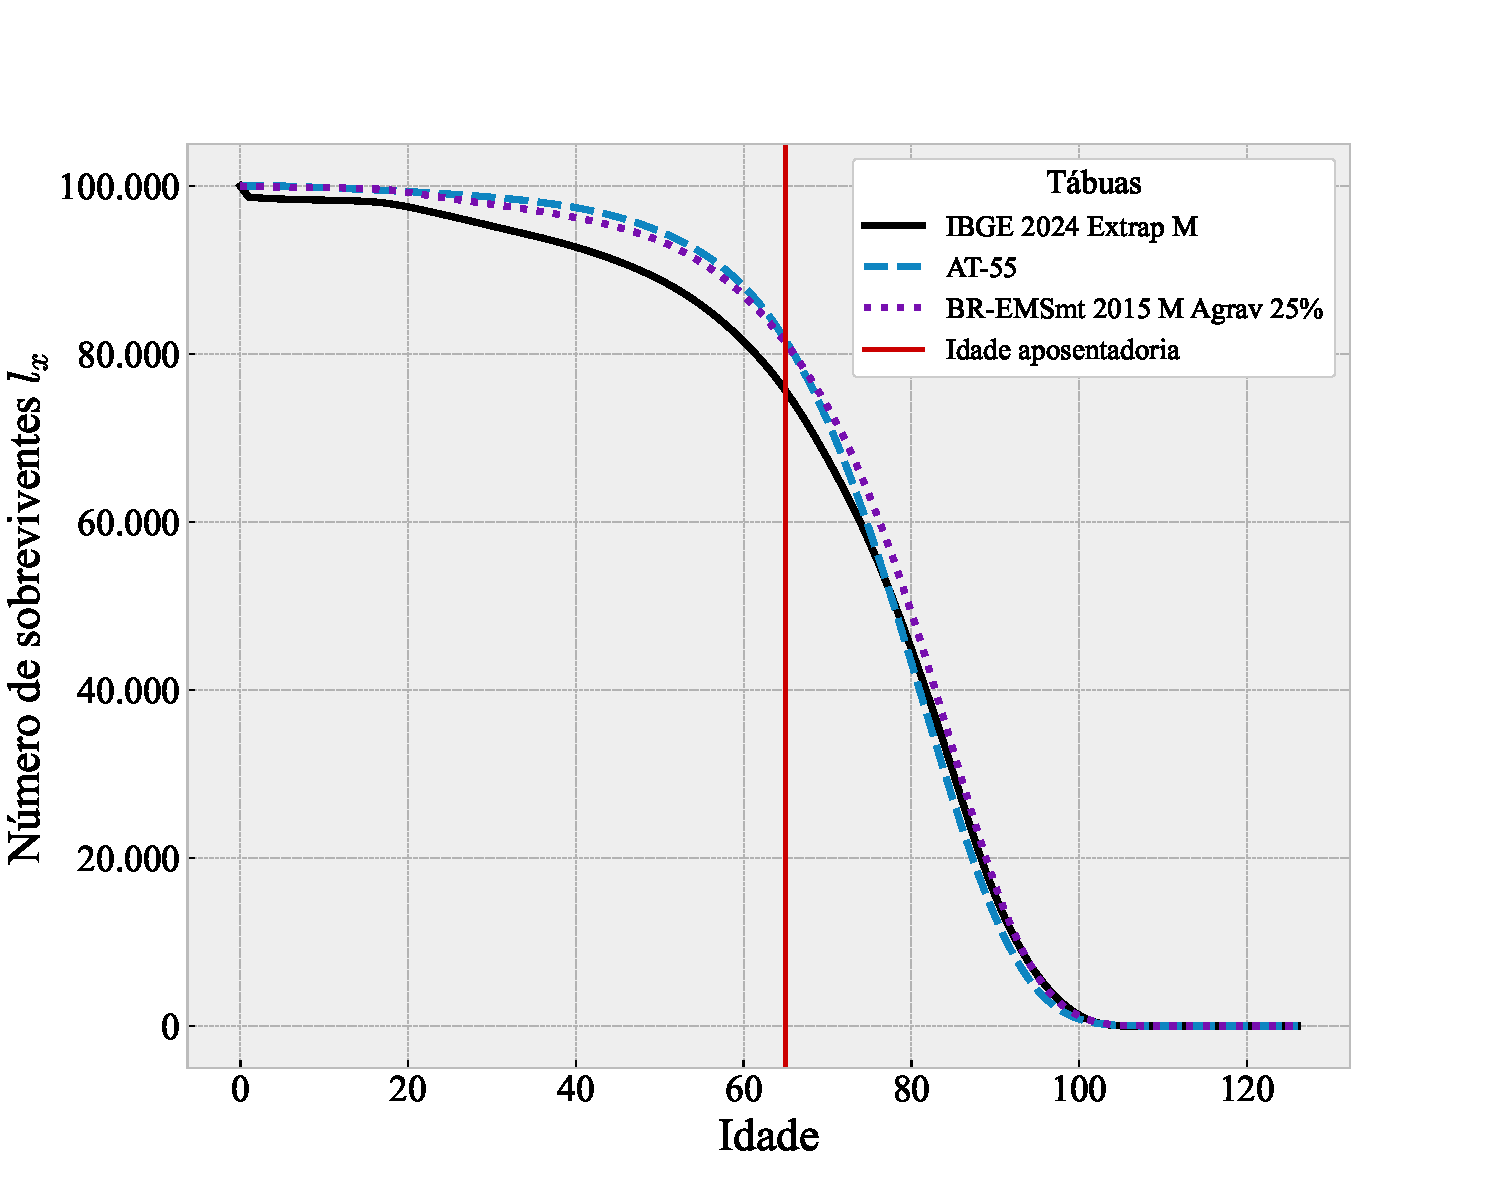
\includegraphics[width=0.84\textwidth, trim=0 0 0 2cm, clip]{curva_lx_masc.pdf}
    \fonte{Elaboração própria (2026).}
    \label{fig:curva_lx_jovem_masc}
\end{figure}

A partir da análise visual da Figura \ref{fig:curva_lx_jovem_masc}, observa-se que tanto a tábua AT-55 quanto a tábua BR-EMSmt 2015 Masculina agravada em 25\% apresentam curvas de $l_x$ semelhantes ao longo de todo o período contributivo. Nesse intervalo de idades, ambas permanecem estritamente acima da curva $l_x$ da tábua IBGE 2024 Extrapolada Masculina, o que indica níveis de sobrevivência mais elevados durante a fase contributiva. 

Consequentemente, espera-se que essas tábuas produzam um VACF superior ao obtido com a tábua de referência. Entretanto, após a idade de 65 anos, observa-se uma mudança no comportamento dessas curvas. A partir desse ponto, as curvas passam a se aproximar e eventualmente se cruzam. No caso da tábua AT-55, a curva $l_x$ apresenta uma queda mais acentuada, passando a situar-se abaixo da curva da tábua IBGE 2024 Extrapolada Masculina por volta da idade 75. Já a curva correspondente à tábua BR-EMSmt 2015 Masculina agravada em 25\% apresenta um declínio mais gradual, aproximando-se da curva da tábua de referência apenas por volta da idade 90, mantendo, contudo, sua superioridade.

Esse comportamento sugere implicações distintas para o VABF. No caso da tábua AT-55, a redução mais acentuada da sobrevivência nas idades avançadas indica que o aumento observado no VACF pode não ser acompanhado por um crescimento proporcional no VABF, uma vez que as probabilidades de sobrevivência durante o período de pagamento dos benefícios torna-se relativamente menor. Em contrapartida, para a tábua BR-EMSmt 2015 Masculina agravada em 25\%, o comportamento da curva $l_x$ nas idades mais elevadas é mais próximo ao da tábua de referência. Assim, o aumento do VACF tende a ser acompanhado por um aumento aproximadamente proporcional no VABF.

\begin{figure}[H]
    \centering
    \singlespacing\caption{Curvas $l_x$ Femininas ao Comparar Diferentes Tábuas}
    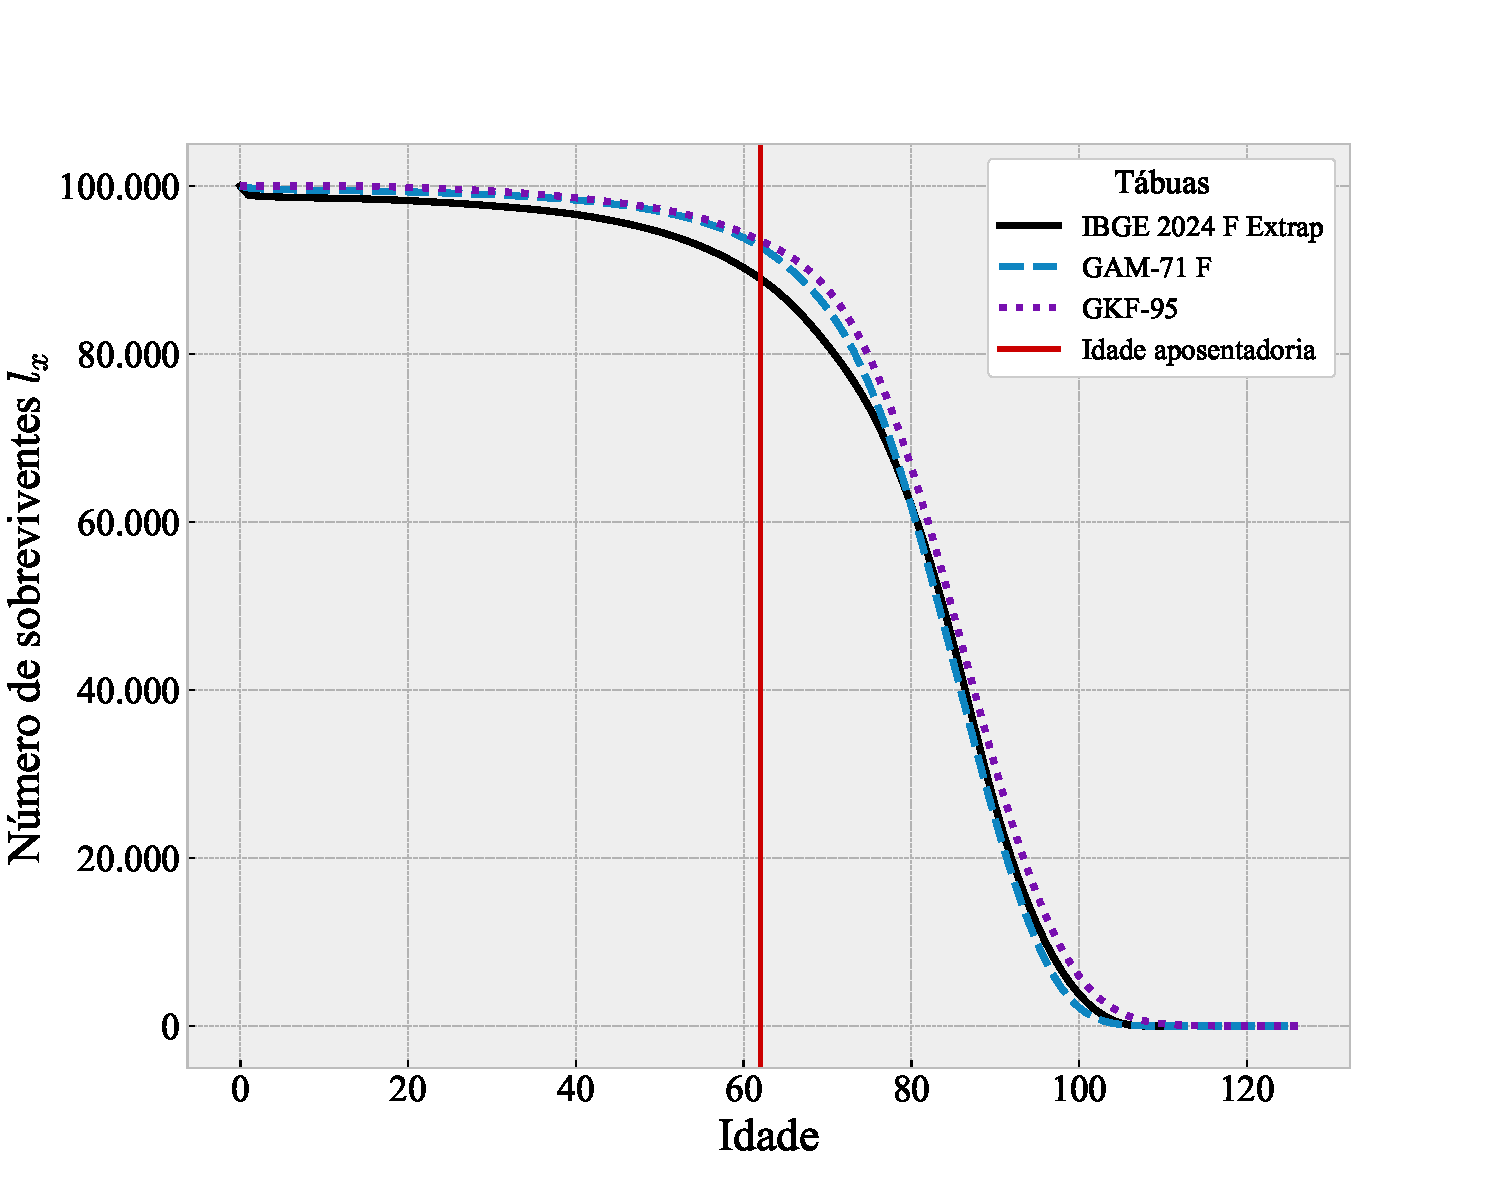
\includegraphics[width=0.84\textwidth, trim=0 0 0 2cm, clip]{curva_lx_fem.pdf}
    \fonte{Elaboração própria (2026).}
    \label{fig:curva_lx_jovem_fem}
\end{figure}

A análise visual da Figura \ref{fig:curva_lx_jovem_fem} apresenta um padrão semelhante ao observado na Figura \ref{fig:curva_lx_jovem_masc}. A tábua GKF-95 mantém sua curva de $l_x$ consistentemente acima da curva da tábua IBGE 2024 Extrapolada Feminina ao longo de todas as idades, aproximando-se da curva da tábua IBGE 2024 Extrapolada Feminina apenas em idade superiores a 85 anos. 

Esse comportamento sugere que o aumento no VACF tende a ser acompanhado por um aumento aproximadamente proporcional no VABF. Por outro lado, a tábua GAM-71 Feminina apresenta um comportamento distinto. Conforme ilustrado na Figura \ref{fig:curva_lx_jovem_fem}, sua curva $l_x$ passa a situar-se abaixo da curva da tábua IBGE 2024 Extrapolada Feminina após os 80 anos. Esse resultado indica que embora possa haver um aumento no VACF durante a fase contributiva, tal aumento não é necessariamente acompanhado por um crescimento proporcional no VABF, devido ao nível relativamente menor de sobrevivência nas idades avançadas.

Portanto, com o índice proposto na Equação \ref{eq:indice}, é possível compreender como os níveis de sobrevivência de $l_x$ são impactados pela distribuição etária da população. Ao calcular os índices referentes aos exemplos de tábuas utilizados na Figura \ref{fig:curva_lx_jovem_masc}, observa-se que a tábua AT-55 apresentou um indicador de aproximadamente $I_{Ativos} = 3,3$ para as idades contributivas, indicando que a tábua comparativa gera um VACF superior àquele obtido pela tábua de referência, o que está em consonância com a discussão realizada na análise visual. 

Essa tábua também apresentou um indicador para as idades de aposentadoria de aproximadamente $I_{Aposentados} = -0,81$, sugerindo que a tábua comparativa gera um VABF inferior ao gerado pela tábua de referência. Por sua vez, a tábua BR-EMSmt 2015 Masculina Agravada em 25\% apresentou indicadores positivos tanto para o período contributivo quanto para o período de aposentadoria, aproximadamente $I_{Ativos} = 2,6$ e $I_{Aposentados}8,6$, respectivamente, indicando que o aumento no VACF foi acompanhado por um aumento no VABF.

Ao analisar os índices calculados para as tábuas GAM-71 e GKF-95, nota-se que os índices da segunda tábua sugerem um VACF maior, acompanhado também de um VABF mais elevado. Nesse caso, os índices observados são de aproximadamente $I_{Ativos} = 1,89$ na fase contributiva e $I_{Aposentados} = 9,04$ nas idades de aposentadoria. Por outro lado, a tábua GAM-71 apresenta um comportamento distinto. O índice de $I_{Ativos} = 1,43$ nas idades contributivas indica que o VACF também é relativamente elevado nessa tábua. Entretanto, nas idades de aposentadoria, o índice observado é de $I_{Aposentados} = 0,61$, sugerindo que o VABF não acompanha, na mesma proporção, o aumento observado no VACF.

As Tabelas \ref{tab:indices_equilibrada_pminf}, \ref{tab:indices_jovem_pminf}, \ref{tab:indices_idosa_pminf} e \ref{tab:indices_bimodal_pminf} apresentam os índices calculados para as fases contributiva e de aposentadoria das tábuas que apresentaram inconsistências nas bases equilibrada, jovem, idosa e bimodal, respectivamente.
\newpage
\begin{table}[htbp]
    \centering
    \caption{Índices da Base Equilibrada para Tábuas com PM Inferior}
    \begin{threeparttable}
    \renewcommand{\arraystretch}{1.0}
    \begin{tabular}{llrr}
    \toprule
    \textbf{Gênero} & \textbf{Tábua} & \textbf{$I_{Ativos}$} & \textbf{$I_{Aposentados}$} \\ 
    \midrule
    \multirow{8}{*}{Masculino} 
        & IBGE 2021 Extrapolada Masculina Suavizada em 1\%      & 0,1860 & -0,2839 \\
        & IBGE 2019 Extrapolada Ambos Agravada em 18,3\%  & 0,8697 &  0,5589 \\
        & AT-2000 Masculina Agravada em 33\%              & 4,0568 &  4,2489 \\
        & AT-55 Suavizada em 5\%                    & 5,5193 &  4,4851 \\
        & AT-83 Basic Masculina Suavizada em 2,5\%          & 6,2039 &  6,3165 \\
        & BR-EMSmt-v.2021 Masculina Agravada em 24\%      & 4,0914 &  4,1542 \\
        & Prudential-50 Suavizada em 16\%           & 5,9100 &  5,0220 \\
        & M-95 H Suavizada em 6\%                   & 1,8742 &  1,2814 \\
    \hline
    \multirow{6}{*}{Feminino}
        & BR-EMSmt-v.2021 Feminina Agravada em 21,5\%    &  1,4900 &  0,8087 \\
        & GAM-71 Feminina Suavizada em 5\%                 &  2,1025 &  4,2357 \\
        & IBGE 2020 Extrapolada Feminina                &  0,2176 & -0,4941 \\
        & IBGE 2019 Extrapolada Ambos Suavizada em 19\% & -1,0670 & -3,3963 \\
        & IBGE 2019 Extrapolada Feminina                &  0,1239 & -1,1209 \\
        & Petros Suavizada em 15\%              &  2,6855 &  2,5947 \\
    \bottomrule
    \end{tabular}
    \begin{tablenotes}[flushleft]
        \small
        \item Fonte: Elaboração própria (2026).
    \end{tablenotes}
    \end{threeparttable}
    \label{tab:indices_equilibrada_pminf}
\end{table}
\vspace{0.5cm}
\begin{table}[htbp]
    \centering
    \caption{Índices da Base Jovem para Tábuas com PM Inferior}
    \begin{threeparttable}
    \renewcommand{\arraystretch}{1.0}
    \begin{tabular}{llrr}
    \toprule
    \textbf{Gênero} & \textbf{Tábua} & \textbf{$I_{Ativos}$} & \textbf{$I_{Aposentados}$} \\ 
    \midrule
    \multirow{12}{*}{Masculino} 
        & IBGE 2019 Extrapolada Ambos Agravada em 19\% & 0,3090 & 0,0375 \\
        & IBGE 2019 Extrapolada Ambos Agravada em 18,3\% & 0,3487 & 0,7004 \\
        & AT-2000 Masculina Agravada em 33\% & 2,1921 & 1,7122 \\
        & AT-55 & 3,3531 & -0,8167 \\
        & AT-55 Suavizada em 5\% & 3,4374 & 2,9086 \\
        & AT-83 Basic Masculina & 3,7035 & 1,6655 \\
        & AT-83 Basic Masculina Suavizada em 2,5\% & 3,7371 & 3,4338 \\
        & BR-EMSmt-v.2021 Masculina Agravada em 24\% & 2,5995 & 2,4447 \\
        & GKM-95 & 2,7029 & -2,4822 \\
        & Prudential-50 Suavizada em 16\% & 3,8411 & 5,0979 \\
        & TR 2025 & 1,6324 & 4,3454 \\
        & M-95 H Suavizada em 6\% & 0,5308 & -0,8540 \\
    \hline
    \multirow{4}{*}{Feminino}
        & BR-EMSmt-v.2021 Feminina Agravada em 21,5\% & 1,2519 & 1,0326 \\
        & GAM-71 Feminina & 1,4372 & 0,6113 \\
        & GAM-71 Feminina Suavizada em 5\% & 1,5006 & 3,1142 \\
        & Petros Suavizada em 13\% & 2,1174 & 0,7493 \\
    \bottomrule
    \end{tabular}
    \begin{tablenotes}[flushleft]
        \small
        \item Fonte: Elaboração própria (2026).
    \end{tablenotes}
    \end{threeparttable}
    \label{tab:indices_jovem_pminf}
\end{table}

\FloatBarrier
A partir da Tabelas \ref{tab:indices_equilibrada_pminf} e \ref{tab:indices_jovem_pminf} observa-se que parte das tábuas inconsistentes segue o padrão verificado nos exemplos anteriores, isto é, $I_{Ativo} > I_{Aposentado}$. Entretanto, também se identificam tábuas inconsistentes que não seguem esse comportamento. Nesses casos, verifica-se $I_{Aposentados} > I_{Ativos}$, ainda assim resultando em uma PM inferior àquela obtida com a tábua de referência, o que evidencia uma limitação do índice proposto. 
\newpage
Tal limitação pode estar associada à complexidade inerente ao cálculo da PM, bem como a determinadas particularidades dos métodos de custeio. Como o índice proposto avalia apenas a tábua de mortalidade, ele não capta a influência das demais premissas atuariais que compõem o cálculo da PM, tampouco do mecanismo de determinação das contribuições. Um exemplo é o método PNI, no qual a premissa de crescimento salarial influencia diretamente o valor das contribuições.
\vspace{0.25cm}
\begin{table}[htbp]
    \centering
    \caption{Índices da Base Idosa para Tábuas com PM Inferior}
    \begin{threeparttable}
    \renewcommand{\arraystretch}{1.0}
    \begin{tabular}{llrr}
    \toprule
    \textbf{Gênero} & \textbf{Tábua} & \textbf{$I_{Ativos}$} & \textbf{$I_{Aposentados}$} \\ 
    \midrule
    \multirow{5}{*}{Masculino} 
        & Prudential-50 Suavizada em 19\% & 6,6859 & 7,6000 \\
        & RP-2000 M               & 9,6269 & 21,665 \\
        & UP - 94 M	               & 8,3839 & 15,369 \\
        & TR 2025                  & 1,9063 & 4,1501 \\
        & Petros                   & 9,6252 & 24,157 \\ \hline
    \multirow{4}{*}{Feminino}
        & AT-83 Basic F  & 3,8171 & 8,8050 \\
        & RP-2000 F  & 3,7881 & 6,2794 \\
        & CL5	 & 3,2476 & 10,7634 \\
        & M-95 M Suavizada em 7\%  & 1,1250 & 1,7197 \\
    \bottomrule
    \end{tabular}
    \begin{tablenotes}[flushleft]
        \small
        \item Fonte: Elaboração própria (2026).
    \end{tablenotes}
    \end{threeparttable}
    \label{tab:indices_idosa_pminf}
\end{table}

No contexto da base idosa, apenas duas tábuas, uma por gênero, produziram PM inferior à da referência nos métodos de custeio INE e PUC. Estas tábuas apresentam $I_{Aposentados} > I_{Ativo} > 0$, indicando que a sobrevivência é superior à da referência em todo o intervalo de idades, com destaque para as idades avançadas. Entretanto, para esse perfil etário com massa de ativos reduzida, mesmo um índice contributivo modesto pode representar um crescimento do VACF suficiente para, em conjunto com o crescimento do VABF, resultar em PM menor. O mecanismo opera, portanto, não pela dominância do VACF sobre o VABF, mas pelo equilíbrio proporcional entre os dois componentes dentro de uma estrutura com poucos ativos.

As demais tábuas apresentadas na Tabela \ref{tab:indices_idosa_pminf} — Prudential-50 Suav. 19\%, TRP-2000 M, UP-94 M, Petros (masculino) e AT-83 Basic F, RP-2000 F, CL5 (feminino) — apresentam índices consideravelmente mais elevados, especialmente no que diz respeito ao $I_{Aposentados}$. Entretanto, essa tábuas só apresentam inconsistências no método de custeio PNI e, portanto, como discutido nos resultados da Tabela \ref{tab:indices_jovem_pminf}, o indicador proposto não é afetado pela premissa de crescimento salarial utilizada no cálculo do VACF nesse método de custeio.

\newpage
\begin{table}[htbp]
    \centering
    \caption{Índices da Base Bimodal para Tábuas com PM Inferior}
    \begin{threeparttable}
    \renewcommand{\arraystretch}{1.0}
    \begin{tabular}{llrr}
    \toprule
    \textbf{Gênero} & \textbf{Tábua} & \textbf{$I_{Ativos}$} & \textbf{$I_{Aposentados}$} \\ 
    \midrule
    \multirow{5}{*}{Masculino} 
        & IBGE 2019 Extrapolada Ambos Agravada em 18,3\% & 0,8839 & 0,8056 \\
        & Prudential-50 Suavizada em 18\%         & 6,5978 & 6,8022 \\
        & RP-2000 M                        & 9,6270 & 21,6652 \\
        & UP - 94 M                        & 8,3840 & 15,3693 \\
        & Petros                           & 9,6252 & 24,1574 \\ \hline
    \multirow{3}{*}{Feminino}
        & AT-83 Basic Feminina      & 3,8171 & 8,8050 \\
        & GAM-71 Feminina Suavizada em 5\%  & 2,9656 & 3,8695 \\
        & RP-2000 Feminina          & 3,7882 & 6,2795 \\
    \bottomrule
    \end{tabular}
    \begin{tablenotes}[flushleft]
        \small
        \item Fonte: Elaboração própria (2026).
    \end{tablenotes}
    \end{threeparttable}
    \label{tab:indices_bimodal_pminf}
\end{table}

Para o contexto da base bimodal as tábuas A IBGE 2019 Extrap. A Agravada 18,3\% e GAM-71 Feminina Suav. 5\%  apresentaram resultados inconsistentes nos métodos INE e CUP. Porém, apenas a tábua IBGE 2019 Extrap. A Agravada 18,3\% apresentou o índice de ativos maior que o índice de aposentados. A GAM-71 Feminina Suav. 5\% apresentou $I_{Aposentados} > I_{Ativos}$, nesse caso, o diferencial de sobrevivência nas idades avançadas não é suficientemente elevado para que o VABF supere o crescimento do VACF impulsionado pelos ativos jovens, resultando em PM inferior nos métodos INE e CUP. Já as tábuas Prudential-50 Suav. 18\%, RP-2000 M, UP-94 M, Petros, AT-83 Basic F e RP-2000 F só apresentam inconsistências no método de custeio PNI, tendo as mesma justificativa das demais tábuas que apresentaram inconsistências nesses método, como com $I_{Aposentados} > I_{Ativos}$.

A Tabela \ref{tab:inconsistencias_br_ems} exemplifica como o mecanismo de suavização/agravamento pode resultar em uma tábua com PM inferior mesmo com expectativa de vida na idade média superior, por meio do indicador proposto, utilizando a tábua BR-EMSmt-v.2021 masculina na base jovem.
\vspace{0.25cm}
\begin{table}[htbp]
    \centering
    \caption{Tábuas com inconsistência observada}
    \begin{threeparttable}
    \renewcommand{\arraystretch}{1.2}
    \begin{tabular}{lrrcc}
    \toprule
    \textbf{Tábua} & $I_{Ativos}$ & $I_{Aposentados}$ \\ \midrule
    BR-EMSmt-v.2021 Masculina & 3,183085 & 22,579169 \\
    BR-EMSmt-v.2021 Masculina Agravada em 10\% & 2,977077 & 14,823639 \\
    BR-EMSmt-v.2021 Masculina Agravada em 15\% & 2,856231 & 10,622265 \\
    BR-EMSmt-v.2021 Masculina Agravada em 20\% & 2,720576 & 6,181995 \\
    BR-EMSmt-v.2021 Masculina Agravada em 24\% & 2,599464 & 2,444722 \\ 
    \bottomrule
    \end{tabular}
    \begin{tablenotes}[flushleft]
        \small
        \item Fonte: Elaboração própria (2026).
    \end{tablenotes}
    \end{threeparttable}
    \label{tab:inconsistencias_br_ems}
\end{table}

A leitura dos índices revela que à medida que o fator de agravamento aumenta de $0\%$ a $24\%$, o $I_{Ativos}$ decresce de forma relativamente contida, de $3,18$ para $2,60$, ao passo que o $I_{Aposentados}$ colapsa de $22,58$ para $2,44$, uma queda de cerca de $89\%$. Essa divergência na taxa de redução dos dois índices é o mecanismo central da inconsistência.

Na tábua sem agravamento, o $I_{Aposentados}$ é aproximadamente sete vezes superior ao $I_{Ativos}$, indicando que o diferencial de sobrevivência da tábua comparativa em relação à referência é substancialmente mais pronunciado nas idades de aposentadoria do que nas idades contributivas. Nesse cenário, o aumento do VABF supera amplamente o aumento do VACF, de modo que a PM resultante é superior à da tábua de referência.

Entretanto, o agravamento progressivo da tábua atua de forma desigual sobre as duas fases do ciclo previdenciário. A mortalidade adicional introduzida pelo fator de agravamento reduz a sobrevivência em todas as idades, mas seu efeito é proporcionalmente muito mais severo nas idades avançadas. Em contrapartida, nas idades contributivas, a diferença entre as curvas $l_x$ da tábua comparativa e da referência é estruturalmente menor, de modo que o agravamento tenha a mesma intensidade. O resultado é que, a cada incremento do fator de agravamento, o $I_{Aposentados}$ encolhe muito mais rapidamente do que o $I_{Ativos}$. Esse exemplo ilustra, portanto, que a inconsistência, isto é, a PM inferior, não é uma propriedade intrínseca da tábua em sua forma original, mas pode ser induzida pelo próprio processo de calibração.

Em resumo, essa seção identificou situações em que tábuas comparativas com expectativa de vida na idade média superior à da tábua de referência produzem PM inferiores. Os resultados revelam uma relação inversa entre a idade média da massa e a frequência dessas inconsistências. Isto é, as bases mais jovens concentraram os maiores números de ocorrências, enquanto as bases mais idosas registram poucos casos. Esse padrão é atribuído ao fato de que, em massas predominantemente contributivas, o excesso de sobrevivência das tábuas comparativas nas idades ativas eleva o VACF sem contrapartida proporcional no VABF, reduzindo a PM.

O método PNI, dentre os três métodos avaliados, apresentou maior propensão a inconsistências em todas as bases — acumulando 30 ocorrências masculinas e 16 femininas, frente a 19 e 9 do INE —, comportamento associado à premissa de crescimento salarial incorporada ao cálculo do VACF. O sexo masculino concentra mais inconsistências na maioria dos cenários, possivelmente em razão da maior variabilidade histórica da mortalidade masculina. Adicionalmente, o processo de calibração por suavização ou agravamento pode induzir inconsistências inexistentes na tábua original, como demonstrado com a BR-EMSmt-v.2021 M, cujo agravamento progressivo reduz o diferencial de sobrevivência nas idades de benefício de forma muito mais acentuada do que nas idades contributivas.

Para explicar o tais resultados, esta seção propõe dois índices — $I_{Ativos}$ e $I_{Aposentados}$ — que mensuram o diferencial acumulado de sobrevivência entre a tábua comparativa e a de referência em cada fase do ciclo previdenciário. Em geral, inconsistências ocorrem quando $I_{Ativos} > I_{Aposentados}$, embora casos com o padrão inverso também sejam identificados, o que evidencia uma limitação do índice. Por considerar apenas a tábua de mortalidade, ele não captura a influência das demais premissas atuariais.